% This file was created by tikzplotlib v0.9.1.
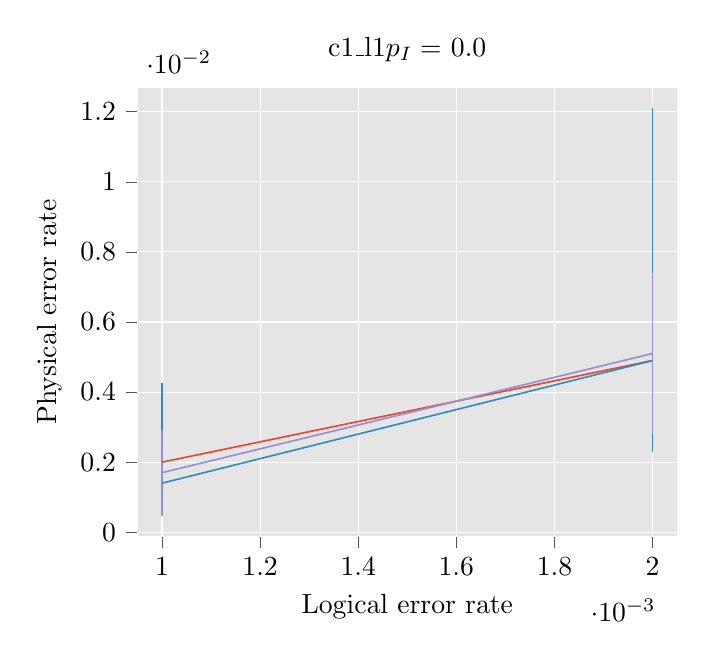
\begin{tikzpicture}

\definecolor{color0}{rgb}{0.886274509803922,0.290196078431373,0.2}
\definecolor{color1}{rgb}{0.203921568627451,0.541176470588235,0.741176470588235}
\definecolor{color2}{rgb}{0.596078431372549,0.556862745098039,0.835294117647059}

\begin{axis}[
axis background/.style={fill=white!89.8039215686275!black},
axis line style={white},
tick align=outside,
tick pos=left,
title={c1\_l1\(\displaystyle p_I = \) 0.0},
x grid style={white},
xlabel={Logical error rate},
xmajorgrids,
xmin=0.00095, xmax=0.00205,
xtick style={color=white!33.3333333333333!black},
y grid style={white},
ylabel={Physical error rate},
ymajorgrids,
ymin=-0.000111743159131897, ymax=0.0126791214662427,
ytick style={color=white!33.3333333333333!black}
]
\path [draw=color0, semithick]
(axis cs:0.001,0.000529904014132316)
--(axis cs:0.001,0.00347009598586769);

\path [draw=color0, semithick]
(axis cs:0.002,0.0026022814712744)
--(axis cs:0.002,0.00719771852872563);

\path [draw=color1, semithick]
(axis cs:0.001,0.00147009598586769)
--(axis cs:0.001,0.0042700959858677);

\path [draw=color1, semithick]
(axis cs:0.002,0.00229771852872561)
--(axis cs:0.002,0.0120977185287256);

\path [draw=color2, semithick]
(axis cs:0.001,0.000469659778385128)
--(axis cs:0.001,0.00293034022161487);

\path [draw=color2, semithick]
(axis cs:0.002,0.00280228147127439)
--(axis cs:0.002,0.00739771852872561);

\addplot [semithick, color0]
table {%
0.001 0.002
0.002 0.00490000000000002
};
\addplot [semithick, color1]
table {%
0.001 0.0014
0.002 0.0049
};
\addplot [semithick, color2]
table {%
0.001 0.0017
0.002 0.0051
};
\end{axis}

\end{tikzpicture}
